\section{Problem Formulation}
\label{sec:formulation}

Given a design brief, the task is to place and style a fixed inventory of
elements on a rectangular canvas. Each brief specifies the canvas dimensions and
background color, an identifier and semantic type for every required element,
verbatim copy or an image description, and design notes. Notes may indicate
target placement zones or describe intended photography to guide image
allocation. We separate constraints that are deterministically verifiable on a
completed layout from qualitative instructions that require design judgment.

\subsection{Shared design state}
A snapshot \(S=(C,E,v)\) comprises a canvas \(C\), an ordered sequence \(E\) of
elements, and an integer version \(v\). The canvas spans
\([0,W]\times[0,H]\) in pixel coordinates with the origin at the upper left.
Each element \(i\) carries a positive-area rectangle
\(R_i=[x_i,x_i+w_i]\times[y_i,y_i+h_i]\), a unique identifier, a semantic type,
and a stacking index \(z_i\); text elements additionally hold copy, font size,
and foreground color, and any element may specify a background fill. Paint order
follows \(z_i\), with later entries in \(E\) drawn above earlier ones on ties.
A valid proposal preserves the brief's canvas, identifiers, types, and required
copy, assigning \(z_i=0\) to card containers and \(z_i>0\) to foreground
elements.

\subsection{Measurable layout constraints}
Let \(F\) denote the foreground elements (excluding card containers) and \(T\)
denote text-bearing elements of type title, subtitle, body, button, or tag. The
overlap rate (OR) measures pairwise foreground intersection area relative to
total foreground area, whereas the boundary overflow rate (BOR) measures the
fraction of elements extending outside the canvas. Writing \(|R|\) for rectangle
area and \(\mathbf{1}[\cdot]\) for an indicator function, we define
\begin{align}
  \mathrm{OR} &= \frac{\sum_{i<j,\;i,j\in F}|R_i\cap R_j|}
                       {\sum_{i\in F}|R_i|}, \label{eq:overlap}\\
  \mathrm{BOR} &= \frac{1}{|E|}\sum_{i\in E}\mathbf{1}[R_i\not\subseteq C].
  \label{eq:overflow}
\end{align}
Shared edges contribute zero intersection area; four coincident equal foreground
boxes yield OR $=6/4$, and BOR counts each overflowing card or foreground box
once.

For each text element \(i\), its effective background is its explicit fill if
specified; otherwise, the detector selects the topmost colored card below \(i\)
in paint order that fully contains \(R_i\), defaulting to the canvas color if no
such card exists. Consequently, moving a text box across a card boundary can
alter its contrast even when all color fields remain unchanged. Let \(L_i^+\)
and \(L_i^-\) be the lighter and darker relative luminances of the text and
effective background colors, computed from linearized sRGB channels. Following
the WCAG contrast formula~\cite{wcag21}, the contrast ratio \(q_i\) and contrast
pass rate (CPR) are
\begin{equation}
 q_i=\frac{L_i^+ + 0.05}{L_i^- + 0.05}, \qquad
 \mathrm{CPR}=\frac{1}{|T|}\sum_{i\in T}\mathbf{1}[q_i\geq\tau_i].
 \label{eq:contrast}
\end{equation}
The benchmark sets \(\tau_i=3.0\) for font sizes of at least 24 pixels and
\(4.5\) otherwise.

The hard constraint satisfaction rate (CSR) averages a binary pass indicator
over tasks, defined for a single snapshot as
\begin{equation}
 \mathrm{CSR}(S)=\mathbf{1}[\mathrm{OR}=0 \land
                         \mathrm{BOR}=0 \land \mathrm{CPR}=1].
 \label{eq:satisfaction}
\end{equation}
On empty sets, OR and BOR equal zero and CPR equals one. Horizontal anchor
alignment (matching left, right, or center edges within 2~px) is tracked offline
and stays tightly clustered across all methods (\vASMin--\vASMax{}). Because
hard checks inspect bounding boxes rather than rendered glyphs, we also compute
an offline raster \emph{text-fit} score: each text element is word-wrapped in
Arial at its assigned font size with $1.2\times$ line spacing and passes if its
rendered width and bottom extent fit within \((w_i,h_i)\); \emph{Hard Fit}
averages the per-brief fraction of passing text elements across hard briefs, and
we also report the layout-level joint rate where both hard checks and all text
elements pass.

\begin{figure*}[t]
\centering
\definecolor{coHubFill}{HTML}{1B365D}
\definecolor{coHubBorder}{HTML}{102340}
\definecolor{coHubHalo}{HTML}{EBF1F8}
\definecolor{coHubHaloLine}{HTML}{9BB0C7}
\definecolor{coHubSub}{HTML}{D8E4F2}
\definecolor{coInk}{HTML}{1C2D40}
\definecolor{coMuted}{HTML}{4F6275}
\definecolor{coStroke}{HTML}{476078}
\definecolor{coReadLine}{HTML}{8196AC}
\definecolor{coNodeFill}{HTML}{F9FBFD}
\definecolor{coBriefFill}{HTML}{F2F5F8}
\definecolor{coDetectFill}{HTML}{EEF3F8}
\definecolor{coTermFill}{HTML}{E3ECF4}
\definecolor{coTermBorder}{HTML}{2A4A6E}
\pgfdeclarelayer{bg}
\pgfsetlayers{bg,main}
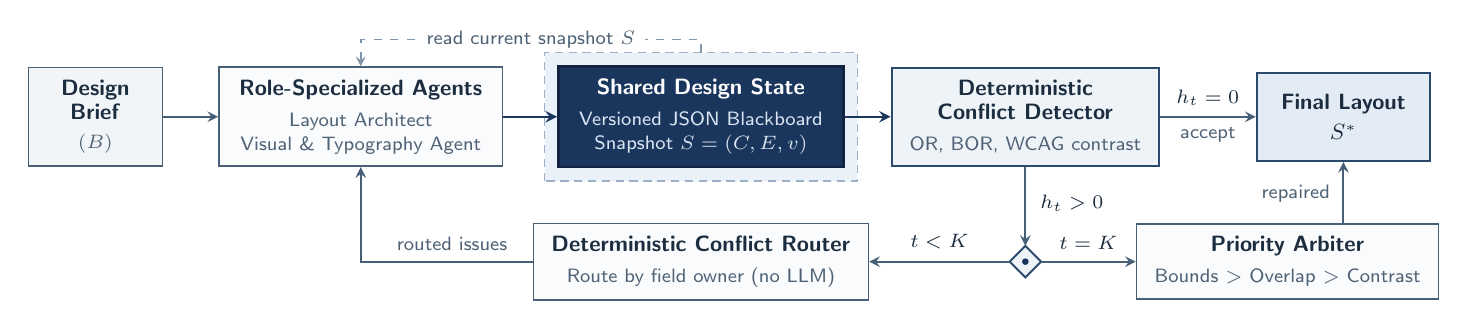
\begin{tikzpicture}[
    x=1cm, y=1cm, font=\sffamily\fontsize{7.6}{9.2}\selectfont,
    boxbase/.style={align=center, inner xsep=6.5pt, inner ysep=4.5pt},
    briefbox/.style={boxbase, draw=coStroke, fill=coBriefFill,
        text=coInk, line width=.58pt, minimum height=1.12cm},
    process/.style={boxbase, draw=coStroke, fill=coNodeFill,
        text=coInk, line width=.62pt, minimum height=1.12cm},
    detectorbox/.style={boxbase, draw=coTermBorder, fill=coDetectFill,
        text=coInk, line width=.68pt, minimum height=1.12cm},
    hubbox/.style={boxbase, draw=coHubBorder, fill=coHubFill,
        text=white, line width=.95pt, minimum height=1.16cm,
        inner xsep=7.5pt, inner ysep=4.6pt},
    terminal/.style={boxbase, draw=coTermBorder, fill=coTermFill,
        text=coInk, line width=.78pt, minimum height=1.12cm},
    flow/.style={draw=coStroke, line width=.70pt, ->, >=stealth},
    hubflow/.style={draw=coHubFill, line width=.85pt, ->, >=stealth},
    readflow/.style={draw=coReadLine, line width=.56pt, dashed, ->, >=stealth},
    cond/.style={font=\sffamily\fontsize{7}{8.2}\selectfont,
        text=coInk, inner sep=1.6pt},
    note/.style={font=\sffamily\fontsize{7}{8.2}\selectfont,
        text=coMuted, inner sep=1.5pt},
    badge/.style={font=\sffamily\fontsize{7}{8.2}\selectfont,
        text=coMuted, fill=white, inner xsep=3.5pt, inner ysep=1.2pt},
]
% Row 1: Brief -> Agents -> Shared Design State (Hub) -> Detector -> Unified Final Layout.
\node[briefbox, minimum width=1.70cm] (brief) at (0.85,0)
    {\textbf{Design}\\[-0.5pt]\textbf{Brief}\\[1.5pt]%
     {\fontsize{7}{8.0}\selectfont\color{coMuted}$(B)$}};
\node[process, minimum width=3.60cm] (agents) at (4.22,0)
    {\textbf{Role-Specialized Agents}\\[2pt]%
     {\fontsize{6.9}{8.2}\selectfont\color{coMuted}Layout Architect}\\[-0.5pt]%
     {\fontsize{6.9}{8.2}\selectfont\color{coMuted}Visual \& Typography Agent}};
\node[hubbox, minimum width=3.40cm] (board) at (8.54,0)
    {\textbf{Shared Design State}\\[2pt]%
     {\fontsize{6.9}{8.2}\selectfont\color{coHubSub}Versioned JSON Blackboard}\\[-0.5pt]%
     {\fontsize{7}{8.2}\selectfont\color{coHubSub}Snapshot $S=(C,E,v)$}};
\node[detectorbox, minimum width=3.20cm] (detector) at (12.66,0)
    {\textbf{Deterministic}\\[-0.5pt]\textbf{Conflict Detector}\\[2pt]%
     {\fontsize{6.9}{8.2}\selectfont\color{coMuted}OR, BOR, WCAG contrast}};
\node[terminal, minimum width=2.20cm] (final) at (16.70,0)
    {\textbf{Final Layout}\\[1.5pt]\textbf{$S^{*}$}};

% Sharp orthogonal outer frame highlighting Shared Design State as the central hub.
\begin{pgfonlayer}{bg}
\fill[coHubHalo]
    ([xshift=-4.5pt,yshift=-4.5pt]board.south west) rectangle
    ([xshift=4.5pt,yshift=4.5pt]board.north east);
\draw[coHubHaloLine, line width=.48pt, densely dashed]
    ([xshift=-4.5pt,yshift=-4.5pt]board.south west) rectangle
    ([xshift=4.5pt,yshift=4.5pt]board.north east);
\end{pgfonlayer}

% Primary Row-1 flow.
\draw[flow] (brief.east) -- (agents.west);
\draw[hubflow] (agents.east) -- (board.west);
\draw[hubflow] (board.east) -- (detector.west);
\draw[flow] (detector.east) --
    node[cond,above=2pt] {$h_t=0$}
    node[note,below=2pt] {accept}
    (final.west);

% Orthogonal blackboard read-back path above Row 1.
\draw[readflow]
    ([yshift=4.5pt]board.north) -- (8.54,0.98) --
    node[badge] {read current snapshot $S$}
    (4.22,0.98) -- (agents.north);

% Row 2: Router (aligned under Hub), Decision Diamond (under Detector), Priority Arbiter.
\node[process, minimum width=3.95cm, minimum height=0.86cm] (critic) at (8.54,-1.84)
    {\textbf{Deterministic Conflict Router}\\[2pt]%
     {\fontsize{6.8}{8.2}\selectfont\color{coMuted}Route by field owner (no LLM)}};
\node[process, minimum width=3.62cm, minimum height=0.86cm] (arbiter) at (15.99,-1.84)
    {\textbf{Priority Arbiter}\\[2pt]%
     {\fontsize{7}{8.2}\selectfont\color{coMuted}Bounds $>$ Overlap $>$ Contrast}};

% Centered decision diamond directly beneath the deterministic conflict detector.
\coordinate (fork) at (12.66,-1.84);
\coordinate (forkN) at (12.66,-1.64);
\coordinate (forkS) at (12.66,-2.04);
\coordinate (forkW) at (12.46,-1.84);
\coordinate (forkE) at (12.86,-1.84);

\draw[flow] (detector.south) --
    node[cond,right=3.5pt,pos=0.46] {$h_t>0$}
    (forkN);
\fill[coDetectFill] (forkN) -- (forkE) -- (forkS) -- (forkW) -- cycle;
\draw[coTermBorder, line width=.70pt] (forkN) -- (forkE) -- (forkS) -- (forkW) -- cycle;
\fill[coHubFill] (fork) circle (1.2pt);

% Branch routing: iterative refinement (t < K) vs. fallback repair merging into Final Layout S*.
\draw[flow] (forkW) -- node[cond,above=2.5pt] {$t<K$} (critic.east);
\draw[flow] (critic.west) -| (agents.south);
\node[note, above=2.5pt] at (5.38,-1.84) {routed issues};
\draw[flow] (forkE) -- node[cond,above=2.5pt] {$t=K$} (arbiter.west);
\draw[flow] (final.south |- arbiter.north) --
    node[note,left=3pt,pos=0.48] {repaired}
    (final.south);
\end{tikzpicture}
\caption{CoLayout control flow. At the start of correction round $t$, the detector counts
$h_t$ hard conflicts on the latest state. The deterministic router dispatches unresolved conflicts
to their field owners (no extra LLM call) while rounds remain. At the round budget $K$, the arbiter applies
repairs in priority order.}
\label{fig:architecture}
\end{figure*}


\section{Proposed Framework}
\label{sec:framework}

\subsection{Role-specific updates to a shared blackboard}
CoLayout coordinates two specialist editing roles through a shared blackboard
and deterministic conflict router (Fig.~\ref{fig:architecture}). During
initialization, the Layout Architect proposes geometry for every required
element, which the system merges with the brief's canvas and copy to build the
first snapshot; the Visual and Typography Agent then reads that snapshot to
initialize font sizes and colors. On subsequent turns, each specialist receives
the brief, the latest snapshot, and only the conflict reports routed to its
role. Every report specifies the conflict type, affected element IDs, severity,
measured magnitude (intersection area in square pixels for overlaps; maximum
overflow protrusion), and a concise description.

Specialists return partial patches keyed by element identifier. Schema
validation restricts geometry patches to position, dimensions, and stacking
index, and visual patches to font size and colors; unknown or non-writable
fields and nested wrappers are rejected and retried rather than silently
dropped. Round-zero style initialization requires explicit foreground colors
and font sizes for every text element and background fills for all card
containers. Each patch is applied to a copy of the current snapshot and
validated against the brief before acceptance; an accepted edit that modifies
any element increments the state version. Logging the pre- and post-patch
versions ties every decision to the exact layout it transformed. Omitted fields
remain intact, allowing the architect to reposition a box without rewriting its
copy or styling.

\subsection{Conflict detection and routing}
Algorithm~\ref{alg:colayout} begins with the two initialization calls in round
zero. In the full framework, the deterministic detector serves as the compliance
critic, emitting a hard report for every positive-area foreground intersection,
canvas overflow, or failed contrast check. If no hard reports are emitted, the
snapshot is accepted immediately. Otherwise, the architect receives all geometry
reports and may update the flagged boxes, after which the visual agent receives
all contrast reports together with the architect's updated snapshot. Each role
is invoked only when assigned at least one issue. Both report sets originate
from the round's initial inspection, and re-inspecting the updated snapshot
catches secondary violations, including contrast regressions across card
boundaries. Anchoring detection to the round-start snapshot establishes clean
round-level audit boundaries and exposes cross-role secondary regressions.

The round counter and state version track distinct events: an empty patch
consumes a correction round without advancing the version, whereas geometry and
style edits within the same round increment the version twice. Tracking rounds
separately ensures a well-defined stopping bound even if a specialist leaves a
reported conflict unresolved.

\begin{algorithm}[t]
\caption{CoLayout with deterministic inspection}
\label{alg:colayout}
\begin{algorithmic}[1]
\Require Design brief \(B\), correction budget \(K\)
\State \(S \gets \Call{InitializeGeometry}{B}\)
\State \(S \gets \Call{InitializeStyle}{B,S}\)
\For{\(t=0,\ldots,K\)}
  \State \(H \gets \Call{HardConflicts}{S}\)
  \If{\(H=\varnothing\)} \State \textbf{break} \EndIf
  \If{\(t=K\)}
     \State \(S \gets \Call{PriorityArbiter}{S}\)
     \State \textbf{break}
  \EndIf
  \For{\(a \in \{\text{Architect},\, \text{Visual}\}\)}
     \State \(H_a \gets \Call{Route}{H,a}\)
     \If{\(H_a\ne\varnothing\)}
        \State \(P \gets \Call{ProposePatch}{a,B,S,H_a}\)
        \State \(S \gets \Call{ValidateAndApply}{S,P}\)
     \EndIf
  \EndFor
\EndFor
\State \Return \(S\) and \(\Call{Evaluate}{S}\)
\end{algorithmic}
\end{algorithm}

\subsection{Priority-ordered repair and ablation}
The correction budget \(K\) bounds the number of specialist revision rounds
after initialization, so an exhaustive run records \(1+K\) rounds. If hard
conflicts persist at the final inspection, the Priority Arbiter executes three
deterministic repair stages in order. First, it resolves canvas overflows by
capping oversized dimensions and clamping box origins inside the canvas. Second,
iterating over overlapping foreground pairs in element order, it evaluates the
minimum translation needed to separate each pair along either axis in both
directions; along the least-displacement axis it attempts an in-bounds shift
that clears all peers, and if neither shift succeeds, it splits the overlapping
interval at its midpoint and crops both boxes to opposite sides. Cropping
preserves disjointness with any peer already separated from the pair.

Third, the arbiter re-evaluates contrast under the repaired geometry and sets
each failing text element to black or white---whichever yields higher contrast.
Within the bounding-box and solid-background model, these stages resolve all
hard conflicts while leaving copy fit to visual inspection, as cropping may
still clip text.

\begin{table*}[t]
\centering
\caption{Eight-method results across 36 briefs $\times$ 3 seeds (108 runs/method, GPT-4o mini). Pre-CSR is pre-arbitration compliance (detector methods reach 100\% terminal CSR under the in-loop check; Sec.~\ref{sec:evaluation}-D reports strict straddling audit); Pre\&Fit adds 100\% pre-arbitration text-fit; Hard Fit is terminal Arial text-fit; Tokens are amortized means; Fail is whole-run failure rate. Bold marks best.}
\label{tab:main}
\small
\setlength{\tabcolsep}{6.0pt}
\begin{tabular}{@{}lrrrrrr@{}}
\toprule
Method & Pre-CSR (\%) $\uparrow$ & Pre\&Fit (\%) $\uparrow$ & Rounds $\downarrow$ & Tokens $\downarrow$ & Hard Fit (\%) $\uparrow$ & Fail (\%) $\downarrow$ \\
\midrule
Single-Agent & 0.0 & 0.0 & \textbf{1.00} & \textbf{2,341} & 93.9 & 3.6 \\
Self-Refine & 5.6 & 5.6 & 4.93 & 9,351 & 92.9 & 4.4 \\
Naive Multi-Agent & 11.1 & 11.1 & 4.30 & 19,893 & 95.1 & 3.6 \\
SA + Det. & 60.2 & 53.7 & 4.02 & 9,467 & \textbf{95.5} & 6.9 \\
SA + BB + Det. & 77.8 & \textbf{63.0} & 3.39 & 5,331 & 94.2 & 2.7 \\
SA-TwoStage + BB + Det. & \textbf{88.0} & 58.3 & 2.98 & 5,548 & 85.8 & \textbf{0.0} \\
\specialrule{0.35pt}{1.5pt}{1.5pt}
Ours w/o Detector & 16.7 & 16.7 & 6.00 & 21,247 & 84.2 & 3.6 \\
CoLayout (Full) & 87.0 & \textbf{63.0} & 2.93 & 5,329 & 85.8 & \textbf{0.0} \\
\bottomrule
\end{tabular}
\end{table*}


The detector ablation (\emph{Ours w/o Detector}) keeps the same blackboard,
permissions, routing, and round budget, substituting an LLM critic on raw JSON.
An empty critic report stops revision early, and remaining reports scope
fallback repair. \mbox{Every} method is scored on its terminal snapshot by the
same evaluator, enabling independent audit of stopping decisions.
